\let\negmedspace\undefined
\let\negthickspace\undefined
\documentclass[journal]{IEEEtran}
\usepackage[a5paper, margin=10mm, onecolumn]{geometry}
%\usepackage{lmodern} % Ensure lmodern is loaded for pdflatex
\usepackage{tfrupee} % Include tfrupee package

\setlength{\headheight}{1cm} % Set the height of the header box
\setlength{\headsep}{0mm}     % Set the distance between the header box and the top of the text

\usepackage{gvv-book}
\usepackage{gvv}
\usepackage{cite}
\usepackage{amsmath,amssymb,amsfonts,amsthm}
\usepackage{algorithmic}
\usepackage{graphicx}
\usepackage{textcomp}
\usepackage{xcolor}
\usepackage{txfonts}
\usepackage{listings}
\usepackage{enumitem}
\usepackage{mathtools}
\usepackage{gensymb}
\usepackage{comment}
\usepackage[breaklinks=true]{hyperref}
\usepackage{tkz-euclide} 
\usepackage{listings}
% \usepackage{gvv}                                        
\def\inputGnumericTable{}                                 
\usepackage[latin1]{inputenc}                                
\usepackage{color}                                            
\usepackage{array}                                            
\usepackage{longtable}                                       
\usepackage{calc}                                             
\usepackage{multirow}                                         
\usepackage{hhline}                                           
\usepackage{ifthen}                                           
\usepackage{lscape}
\usepackage{circuitikz}
\tikzstyle{block} = [rectangle, draw, fill=blue!20, 
    text width=4em, text centered, rounded corners, minimum height=3em]
\tikzstyle{sum} = [draw, fill=blue!10, circle, minimum size=1cm, node distance=1.5cm]
\tikzstyle{input} = [coordinate]
\tikzstyle{output} = [coordinate]


\begin{document}

\bibliographystyle{IEEEtran}
\vspace{3cm}

\title{1.7.3}
\author{AI25BTECH11017-SAI CHARAN}
 \maketitle
% \newpage
% \bigskip
{\let\newpage\relax\maketitle}
\renewcommand{\thefigure}{\theenumi}
\renewcommand{\thetable}{\theenumi}
\setlength{\intextsep}{10pt} % Space between text and floats
\numberwithin{equation}{enumi}
\numberwithin{figure}{enumi}
\renewcommand{\thetable}{\theenumi}
\textbf{Question}:\\
Show that the points $A(-2\hat{i} + 3\hat{j} + 5\hat{k}), \; 
B(\hat{i} + 2\hat{j} + 3\hat{k}), \; 
\text{and } C(7\hat{i} - \hat{k})$ are collinear.
\\ 
\solution \\
Let us solve the given equation theoretically and then verify the solution computationally \\
According to the question, \\
Given position vectors,
\begin{align}
    \vec{A}=\begin{myvec}{-2\\3\\5}\end{myvec}\;
    \vec{B}=\begin{myvec}{1\\2\\3}\end{myvec}\;
    \vec{C}=\begin{myvec}{7\\0\\-1}\end{myvec}\;
\end{align}
To show that these are points are collinear,we show that echolon matrix $\vec{S}$ Rank=1\\

\begin{align}
    \vec{S}=\begin{myvec}{\vec{B}-\Vec{A}&&\vec{C}-\vec{A}}^T\end{myvec}
\end{align}
\begin{align}
    \vec{S}=\begin{myvec}{3&&-1&&-2\\9&&-3&&-6}\end{myvec}
\end{align}


By doing $R_2$=$R_2$-3$R_1$ we get \\
\begin{align}
   \vec{S}=\begin{myvec}{3&&-1&&-2\\0&&0&&0}\end{myvec}
\end{align}
So the Rank of matrix $\vec{S}$ is 1\\
$\therefore$ The points are collinear.

\newpage
\vspace*{0.25cm}

From the figure it is clearly verified that the theoretical solution matches with the computational solution.\\
\begin{figure}[h!]
    \centering
    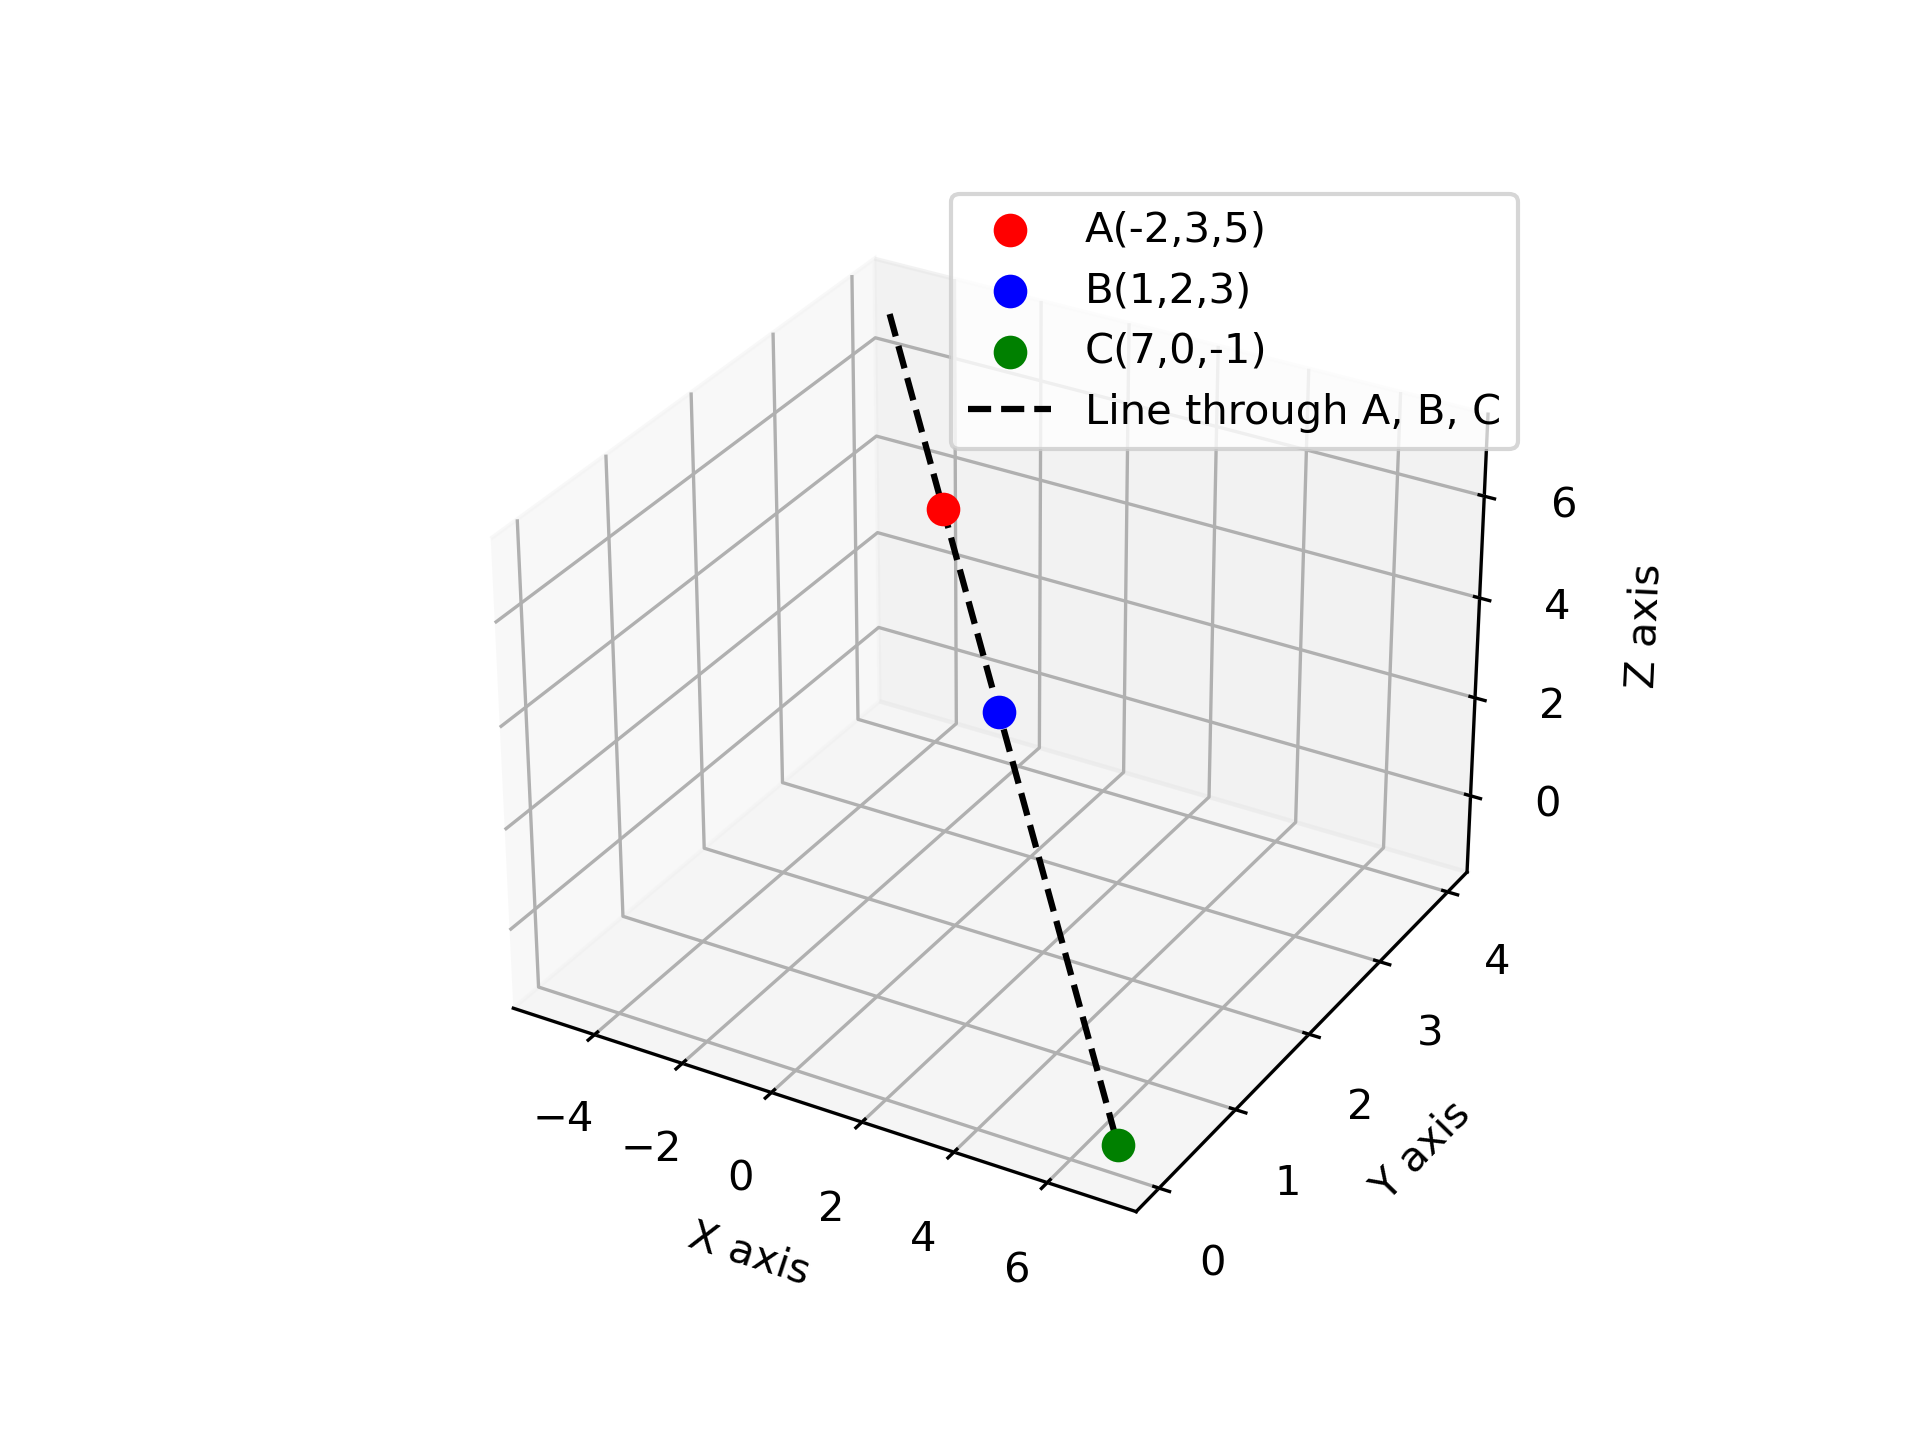
\includegraphics[height=0.5\textheight, keepaspectratio]{figs/fig.png}
    \label{figure_1}
\end{figure}
 


\end{document}